\documentclass[10pt,twocolumn]{article}

\usepackage[margin=0.75in]{geometry}
\usepackage[T1]{fontenc}
\usepackage{lmodern}
\usepackage{helvet}
\usepackage{microtype}
\usepackage{amsmath,amssymb,amsthm}
\usepackage{graphicx}
\usepackage{booktabs}
\usepackage{cite}
\usepackage{xurl}
\usepackage[hidelinks]{hyperref}
\usepackage{titlesec}
\usepackage{caption}
\usepackage{subcaption}
\usepackage{balance}
\usepackage{abstract}
\usepackage{enumitem}

% Column and paragraph spacing
\setlength{\columnsep}{0.24in}
\setlength{\parindent}{1em}
\setlength{\parskip}{0pt}

% Prevent overflow
\sloppy
\emergencystretch=1em
\hyphenpenalty=1000
\tolerance=2000

% Float tuning
\renewcommand{\topfraction}{0.95}
\renewcommand{\bottomfraction}{0.95}
\renewcommand{\textfraction}{0.05}
\renewcommand{\floatpagefraction}{0.9}

% Section styling
\titleformat{\section}{\normalfont\large\bfseries}{\thesection}{1em}{}
\titleformat{\subsection}{\normalfont\normalsize\bfseries}{\thesubsection}{1em}{}
\titleformat{\subsubsection}{\normalfont\normalsize\bfseries}{\thesubsubsection}{1em}{}

% Abstract styling
\renewcommand{\abstractnamefont}{\normalfont\large\bfseries}
\renewcommand{\abstracttextfont}{\normalfont\normalsize}
\setlength{\absleftindent}{0pt}
\setlength{\absrightindent}{0pt}
\setlength{\abstitleskip}{-1em}

% Caption styling
\captionsetup{font=small,labelfont=bf}
\captionsetup[subfigure]{font=small}

\title{
    \textbf{Energy-Efficient Multi-Modal LLM Serving:\\A Sub-phase Characterization Study}
}

\author{
\large
Aashrith Attelli \quad
Amaury Jayr \quad
Nathan Lemma \quad
Mahin Naveen\\[5pt]
\itshape University of Texas at Austin
}

\date{}

\begin{document}

\maketitle

\begin{abstract}
\noindent
Multimodal Large Language Models (MLLMs) are deployed as monolithic pipelines that allocate the full GPU to every inference phase, despite the fact that vision encoding, prefill, and decode have fundamentally different compute and memory demands. We profile the phase differences on InternVL3 by measuring per-phase SM and DRAM throughput. Then, we experiment on sweeping active Streaming Multiprocessor (SM) count from 1 to 108 across batches 1–16 on two workloads: input-heavy and output-heavy. Three results emerged. First, \textbf{decode dominates wall-clock time} (89\% at batch size 1) while sustaining only 14\% SM throughput and 23\% DRAM throughput, leaving substantial measurable headroom on both axes. Second, \textbf{output-heavy throughput plateaus} by SM=36 across every batch size we tested (adding the remaining 67\% of the GPU yields under 9\% additional throughput) while \textbf{input-heavy throughput continues scaling} through SM=108. Third, GPU power saturates at ~230W at the same SM=36 threshold regardless of workload or batch size, which could mean \textbf{single-job SM masking cannot recover the stranded capacity}: the GPU doesn't reach TDP. Batching heavily decreases energy per request for output-heavy workloads (a 13× efficiency between batch 1 to 16) while input-heavy workloads have a smaller effect (2x efficiency) as vision encoder requests do not amortize. We applied spacial partitioning on single-jobs to understand the effects, and hope to motivate future research on complimentary phase inference execution using SM masking.
\end{abstract}

\section{Introduction}

Multi-modal large language models (MLLMs) are models that have the ability to process inputs of many modalities, such as images, audio, or video. Today’s serving frameworks typically run the entire inference pipeline under a single, fixed GPU configuration, even though different stages of the model place very different demands on the hardware. In the models we study, inference breaks down into four main phases: encode, MLP, prefill, and decode.

The encode phase converts each modality into embeddings, with modalities such as vision and audio each having their own processing sub-phases. The MLP stage projects these embeddings into the transformer hidden dimension. Prefill builds the KV-cache for the prompt, and Decode performs autoregressive token generation.

Running all of these phases under one uniform hardware setting leads to mismatches: memory-bound stages end up with more SMs than they can effectively use, while compute-bound stages remain constrained by available processing power. Powering unused hadware units can waste energy and limit serving scalability. A modular serving approach, one that adjusts hardware resources such as SM allocation and device frequency according to the needs of each inference sub-phase, can address this inefficiency.

\section{Background}

MLLM inference is computationally intensive and increasingly costly to serve in production. Recent serving systems exploit phase heterogeneity to improve performance. \textsc{ModServe} time-multiplexes vision encoder and language model on shared GPUs to raise throughput \cite{modserve2025}, and \textsc{CornServe} disaggregates encoder and decoder across separate accelerator pools to reduce tail latency \cite{cornserve2025}, and \textsc{ElasticMM} extends these ideas to cluster-level scheduling, balancing stage workload across multiple workers to address queuing delays and vision encoder bottlenecks \cite{elasticmm2025}. All three treat phase heterogeneity as a scheduling problem: how to place and overlap phases across GPUs and clusters. None measure how each phase actually uses the GPU it has been assigned, and none characterize whether GPU resources are being wasted within a single inference request. 

To achieve disaggregation beyond time-multiplexing, we explore spacial-multiplexing, unexplored in past research. We used SM masking over the traditional Multi-Instance GPU (MIG) or Multi-Process Service (MPS) spacial partitioning options as it gives granular control of processor execution that is necessary for dynamic workload allocation \cite{libsmctrl2023}. 

\section{Motivation}
\label{sec:Motivation}

We first need to understand how much hardware each phase actually utilizes on a single GPU before deciding how to schedule inference phases across GPUs. If different sub-phases use a small portion of compute or a small portion of memory, there could be an opportunity to collocate jobs on the same GPU. To motivate the idea of complimentary phase execution, we conduct a phase-level profile of InternVL3-8B. The goal is to understand the computational and memory differences between the sub-phases and whether the resulting resource demands leave meaningful headroom on either axis.

\begin{figure}[b]
    \centering
    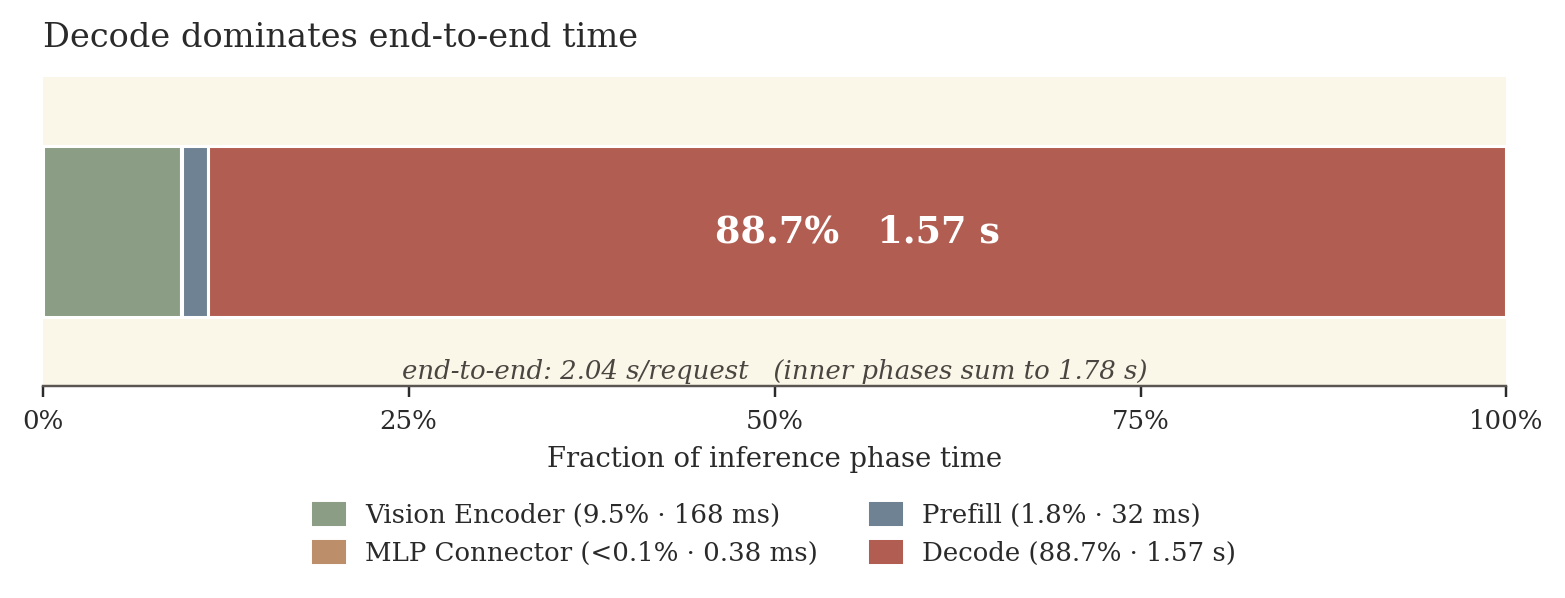
\includegraphics[width=\columnwidth]{figs/fig1a_walltime.png}
    \caption{Wall-time breakdown of a single InternVL3-8B inference
    request (BS=1, $1344^2$ image, 64 output tokens). Decode
    accounts for 88.7\% of phase-attributed runtime.}
    \label{fig:walltime}
\end{figure}

\subsection{Methodology}
We profile InternVL3-8B served through a patched vLLM on a single NVIDIA A100 GPU, with GPU memory utilization fixed at 90\%. To attribute work from the four phases, we add NVTX ranges. These ranges are CPU-side push/pop pairs so reported NVTX times reflect CPU-observed windows rather than GPU-busy time to preserve throughout.

For kernel-level utilization we use Nsight Compute, capturing per-kernel SM throughput and DRAM throughput for the first 200 kernels of Vision, Prefill, and Decode and the first 50 kernels of the much shorter MLP Connector. The reported per-phase numbers in Figure~\ref{fig:utilization} are arithmetic means across these kernels.

The workload is a $\sim$500-token text prompt paired with a $1344 \times 1344$ image, which InternVL3's dynamic tiling expands into approximately $\sim$2560 image tokens. Output length is fixed at 64 tokens and we set the batch to 1. Each configuration runs four warm up requests followed by one profiled request, repeated three times. 

\begin{figure}[t]
    \centering
    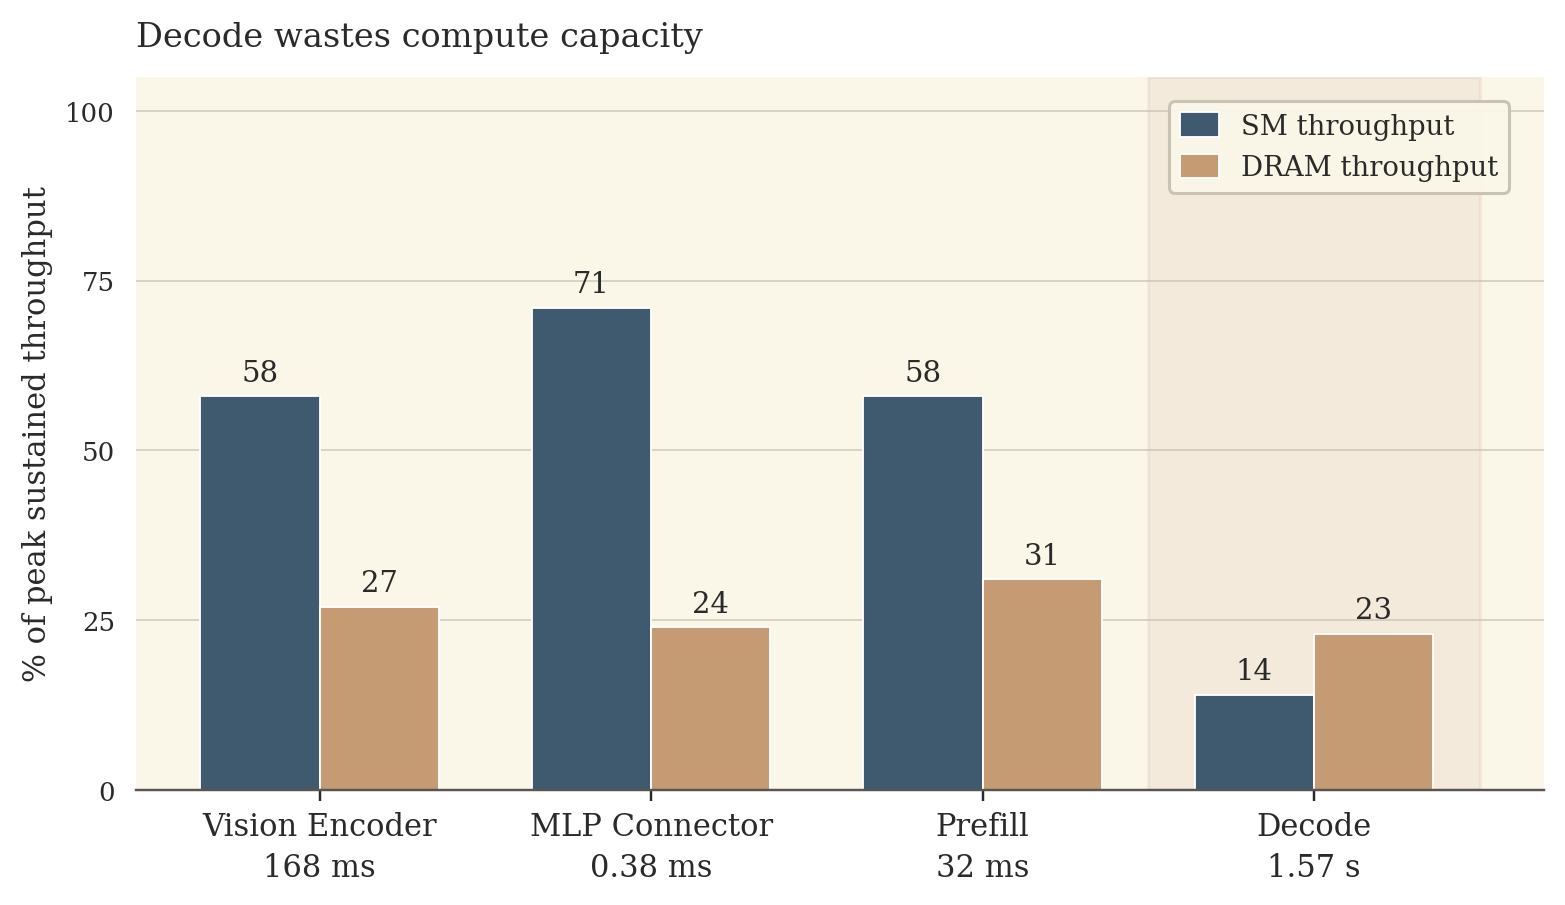
\includegraphics[width=\columnwidth]{figs/fig1b_utilization.png}
    \caption{Wall-time breakdown of a single InternVL3-8B inference
    request (BS=1, $1344^2$ image, 64 output tokens). Decode
    accounts for 88.7\% of phase-attributed runtime.}
    \label{fig:utilization}
\end{figure}

\begin{figure*}[t]
    \centering
    \begin{subfigure}[t]{0.48\textwidth}
        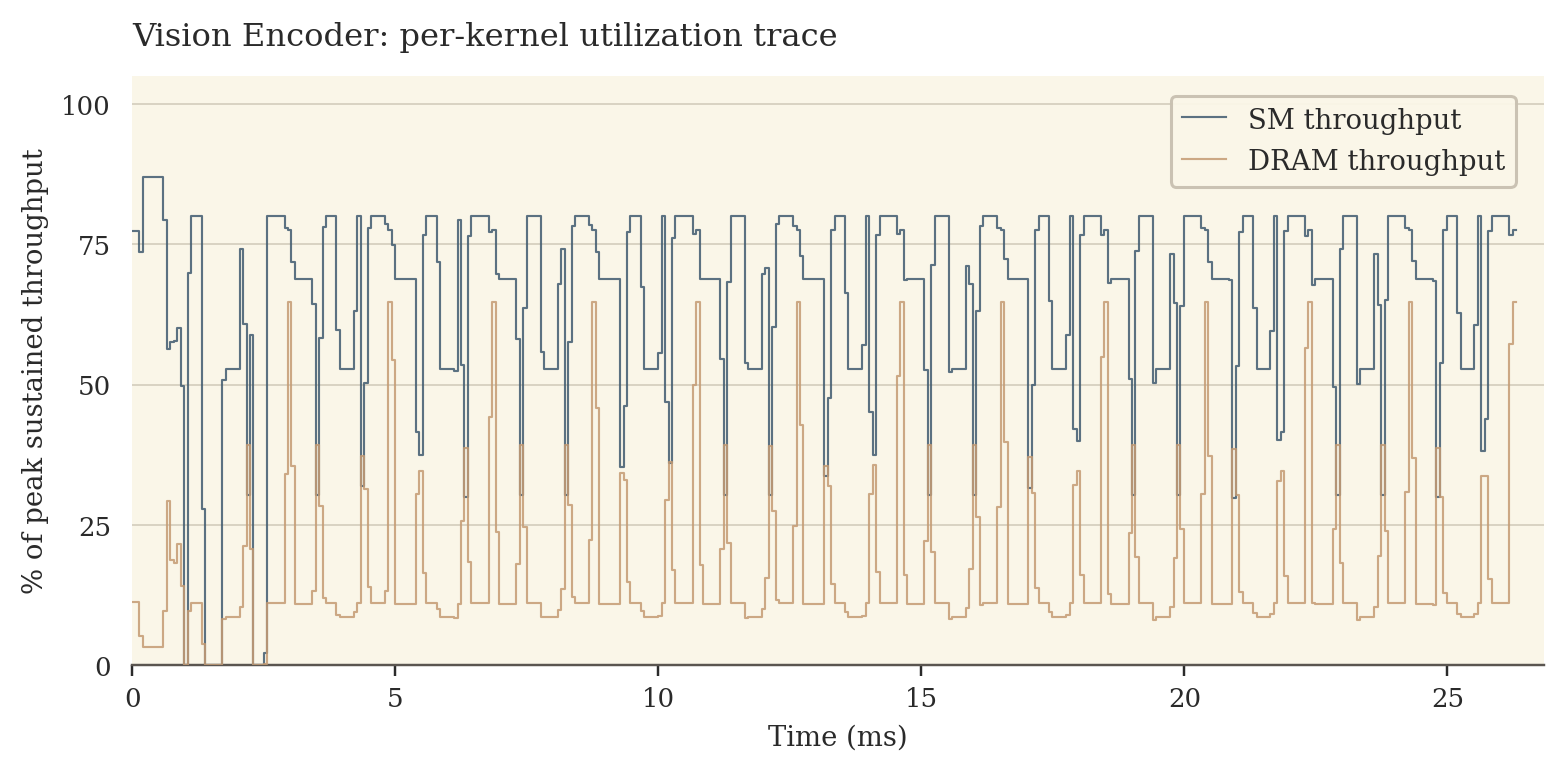
\includegraphics[width=\textwidth]{figs/fig_trace_vision.png}
        \caption{Vision Encoder}
        \label{fig:trace_vision}
    \end{subfigure}
    \hfill
    \begin{subfigure}[t]{0.48\textwidth}
        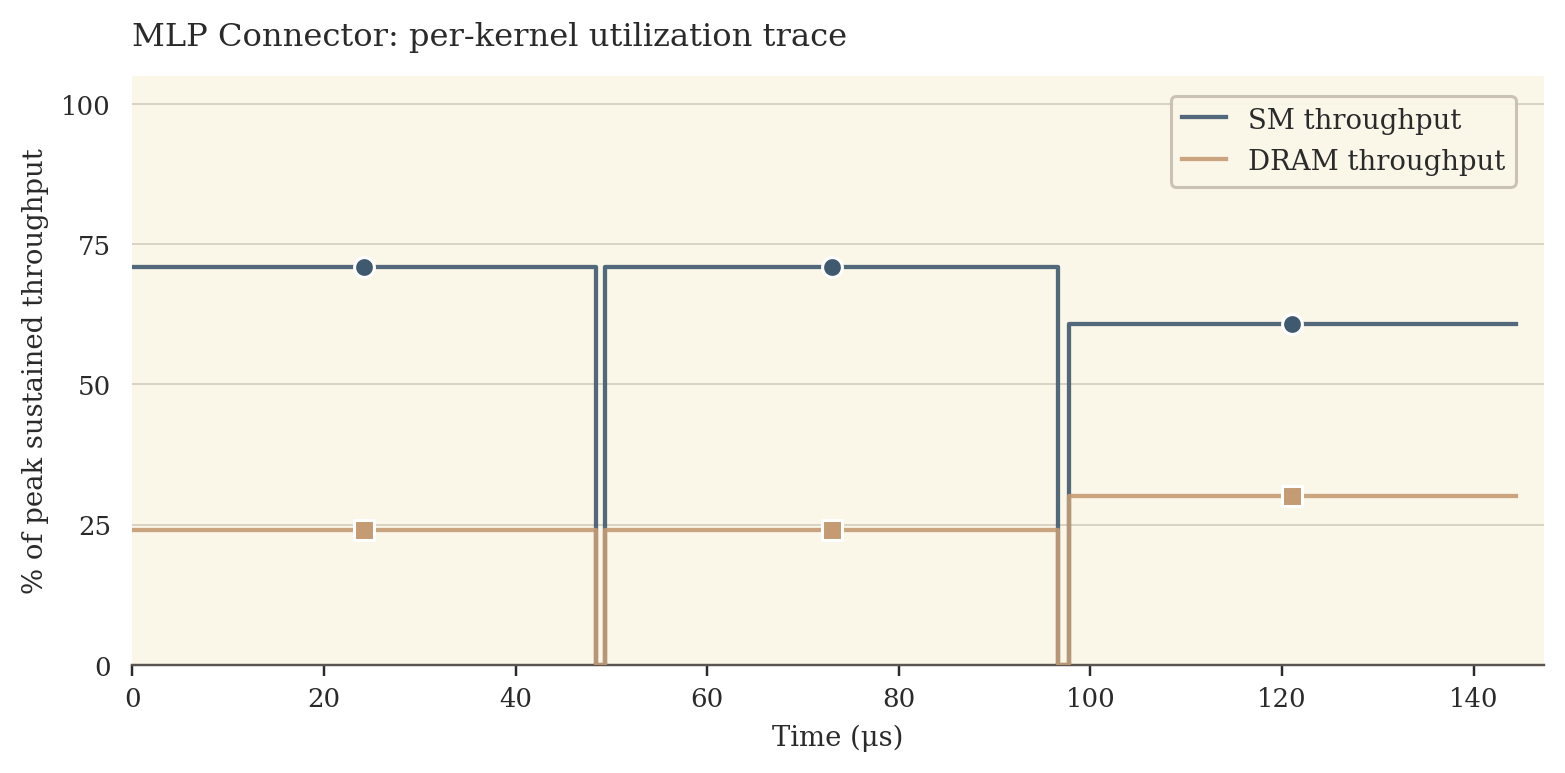
\includegraphics[width=\textwidth]{figs/fig_trace_mlp.png}
        \caption{MLP Connector}
        \label{fig:trace_mlp}
    \end{subfigure}

    \vspace{0.5em}

    \begin{subfigure}[t]{0.48\textwidth}
        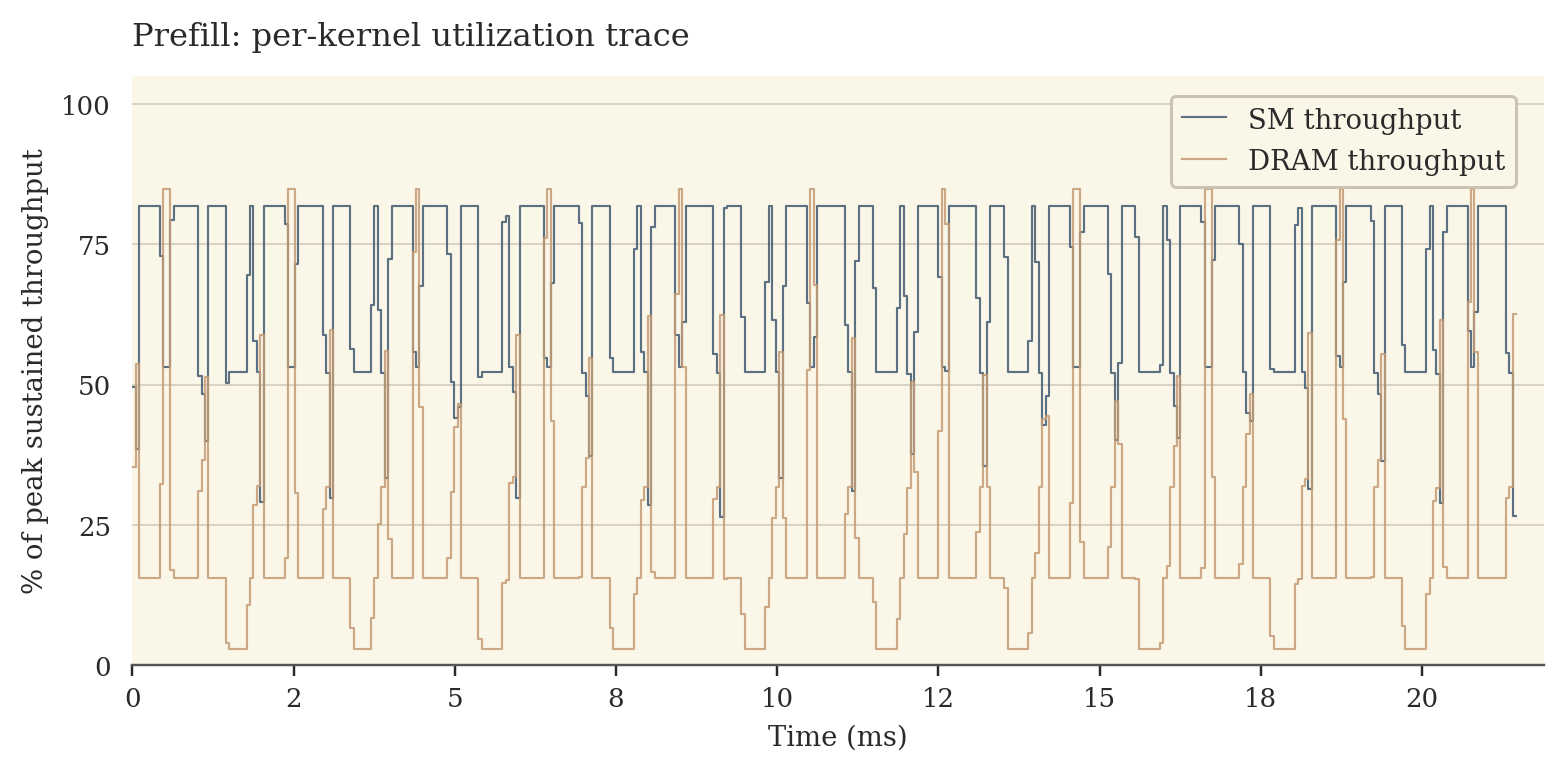
\includegraphics[width=\textwidth]{figs/fig_trace_prefill.png}
        \caption{Prefill}
        \label{fig:trace_prefill}
    \end{subfigure}
    \hfill
    \begin{subfigure}[t]{0.48\textwidth}
        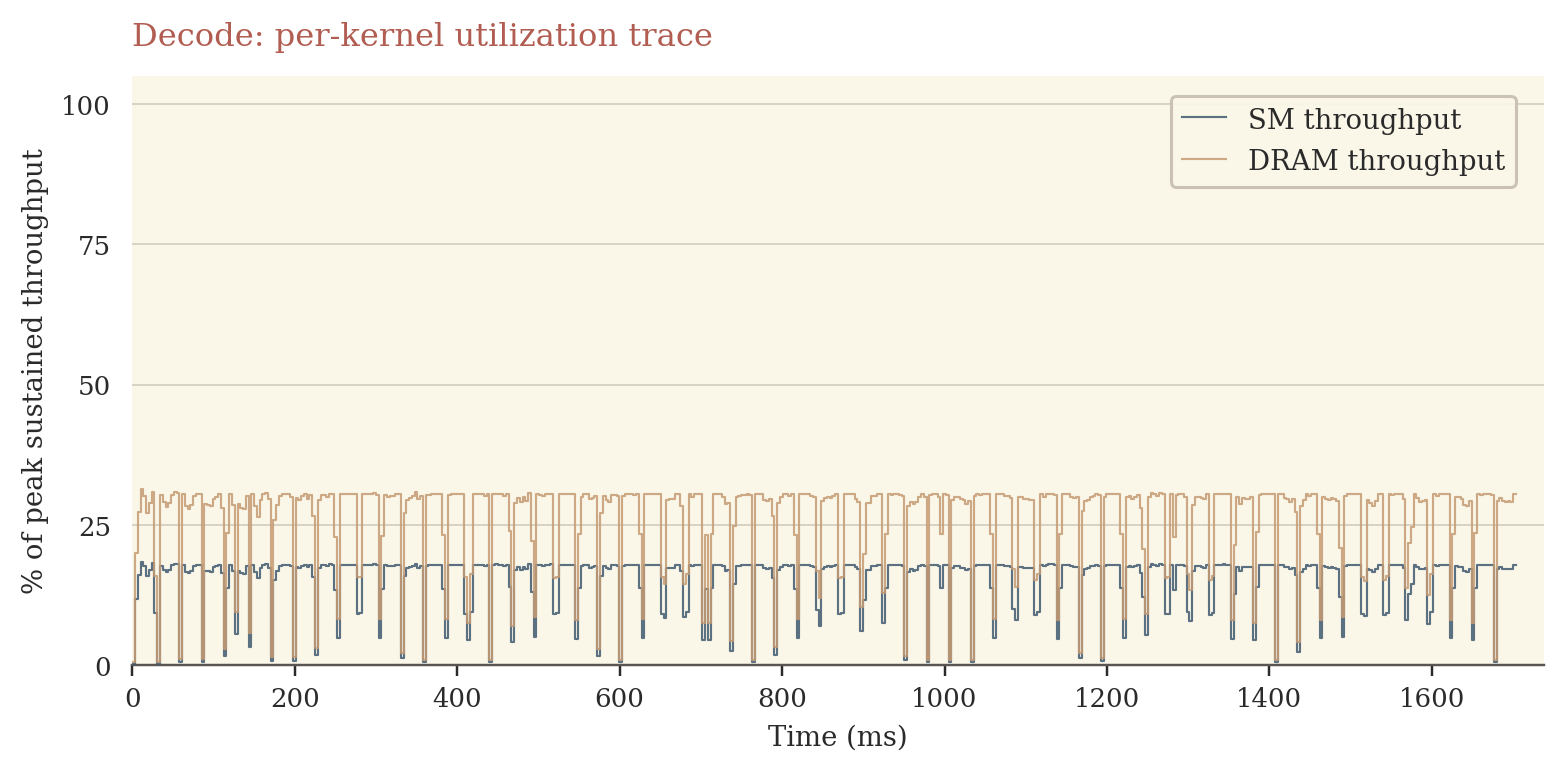
\includegraphics[width=\textwidth]{figs/fig_trace_decode.png}
        \caption{Decode}
        \label{fig:trace_decode}
    \end{subfigure}

    \caption{Per-kernel SM and DRAM throughput traces over the
    duration of each phase. Vision Encoder, MLP Connector, and
    Prefill sustain high SM throughput with periodic DRAM spikes;
    Decode hovers near 14\% SM and 25\% DRAM throughout its
    1.5-second runtime.}
    \label{fig:kernel_traces}
\end{figure*}

\subsection{Decode dominates but underutilizes GPU}

Figure~\ref{fig:walltime} shows the wall-time of a single inference request. Decode accounts for 88.7\% of the time spent. Vision Encoder takes 9.5\%, Prefill 1.8\%, and the MLP Connector is negligible at less than 1\%.

Figure~\ref{fig:utilization} shows what each phase is actually doing with the GPU during that time. Vision Encoder, MLP Connector, and Prefill all sustain high SM throughput with moderate DRAM throughput. Decode is underutilized in both dimensions. The phase that consumes the most time is also the phase that uses the GPU least efficiently.

The kernel-level traces in Figure~\ref{fig:kernel_traces} reinforce this. Vision Encoder \ref{fig:trace_vision} and Prefill \ref{fig:trace_prefill} sustain SM throughput in the 50-80\% range with DRAM regularly spiking to 40-65\%. Decode \ref{fig:trace_decode} is different as SM throughput hovers at $\sim$15\% and DRAM at $\sim$25\% for the entire runtime. Running these phases sequentially under one static GPU configuration means the hardware spends 88.7\% of every request clocked and powered for compute work that is barely happening.

\subsection{Batching cannot reliably close the gap}

A natural question is whether batching closes the utilization gap. At the kernel level, larger decode batches amortize weight loads across concurrent sequences and pull both SM and DRAM throughput higher. This is a well-established result for text-only LLMs that extends to multimodal decode. We do not re-derive it here.

However, batching depends on having batchable concurrent requests, and production multi-modal traffic does not reliably supply them. ModServe's analysis of an Azure production LMM cluster reports a heavy-tailed image-text request distribution (power-law $\alpha=4.4$) with image-driven bursts that are largely uncorrelated with text traffic and have a 79\% prediction error rate when using LLM-tuned forecasting methods~\cite{modserve2025}.

The workloads experienced by production traffic are usually small requests with unpredictable bursts of larger ones and the decode batches are small. Batching helps when traffic permits it but it cannot be the only knob.

\subsection{Summary}

Three observations frame the rest of the paper. First, decode is the longest and most energy-consuming phase of multimodal inference and is also the phase with the most reclaimable headroom on both compute and memory. Second, the other three phases (Vision Encoder, MLP Connector, Prefill) cluster as compute-leaning workloads that already use the GPU effectively. Third, batching cannot close the gap in interactive small-batch regimes. These three facts together motivate the question we evaluate next: if we constrain the compute resource that decode is barely using, does throughput hold up? And if so, can the saved capacity translate into energy savings?

\section{Workloads and Experimental Setup}

We evaluate two workload classes representative of common serving scenarios:

\begin{itemize}[leftmargin=1em]
    \item \textbf{Input-Heavy:} multimodal inference dominated by image processing and prompt construction.
    \item \textbf{Output-Heavy:} decode-heavy autoregressive generation dominated by sustained token production.
\end{itemize}

The Input-Heavy workload uses large multimodal prompts consisting of a $1344\times1344$ image and text inputs with relatively short outputs.

The Output-Heavy workload instead emphasizes sustained autoregressive Decode behavior with longer generated outputs. 
We evaluate each workload across batch sizes 1, 2, 4, 8 and 16.

For every configuration, SM count is swept from 2 SMs to the full 108 SM capacity of the GPU.

Each datapoint represents the average across five independent runs. Experiments follow a closed-loop request pattern to maintain stable runtime conditions during profiling.

For each configuration, we measure average latency, throughput, average GPU power consumption and energy per request.

\section{Evaluation}
Section~\ref{sec:Motivation} established that decode dominates wall time while underutilizing the GPU on both compute and memory dimensions. We now evaluate how throughput, power, and energy respond when the SM allocation itself is constrained, sweeping across all SMs.

\begin{figure}[t]
    \centering
    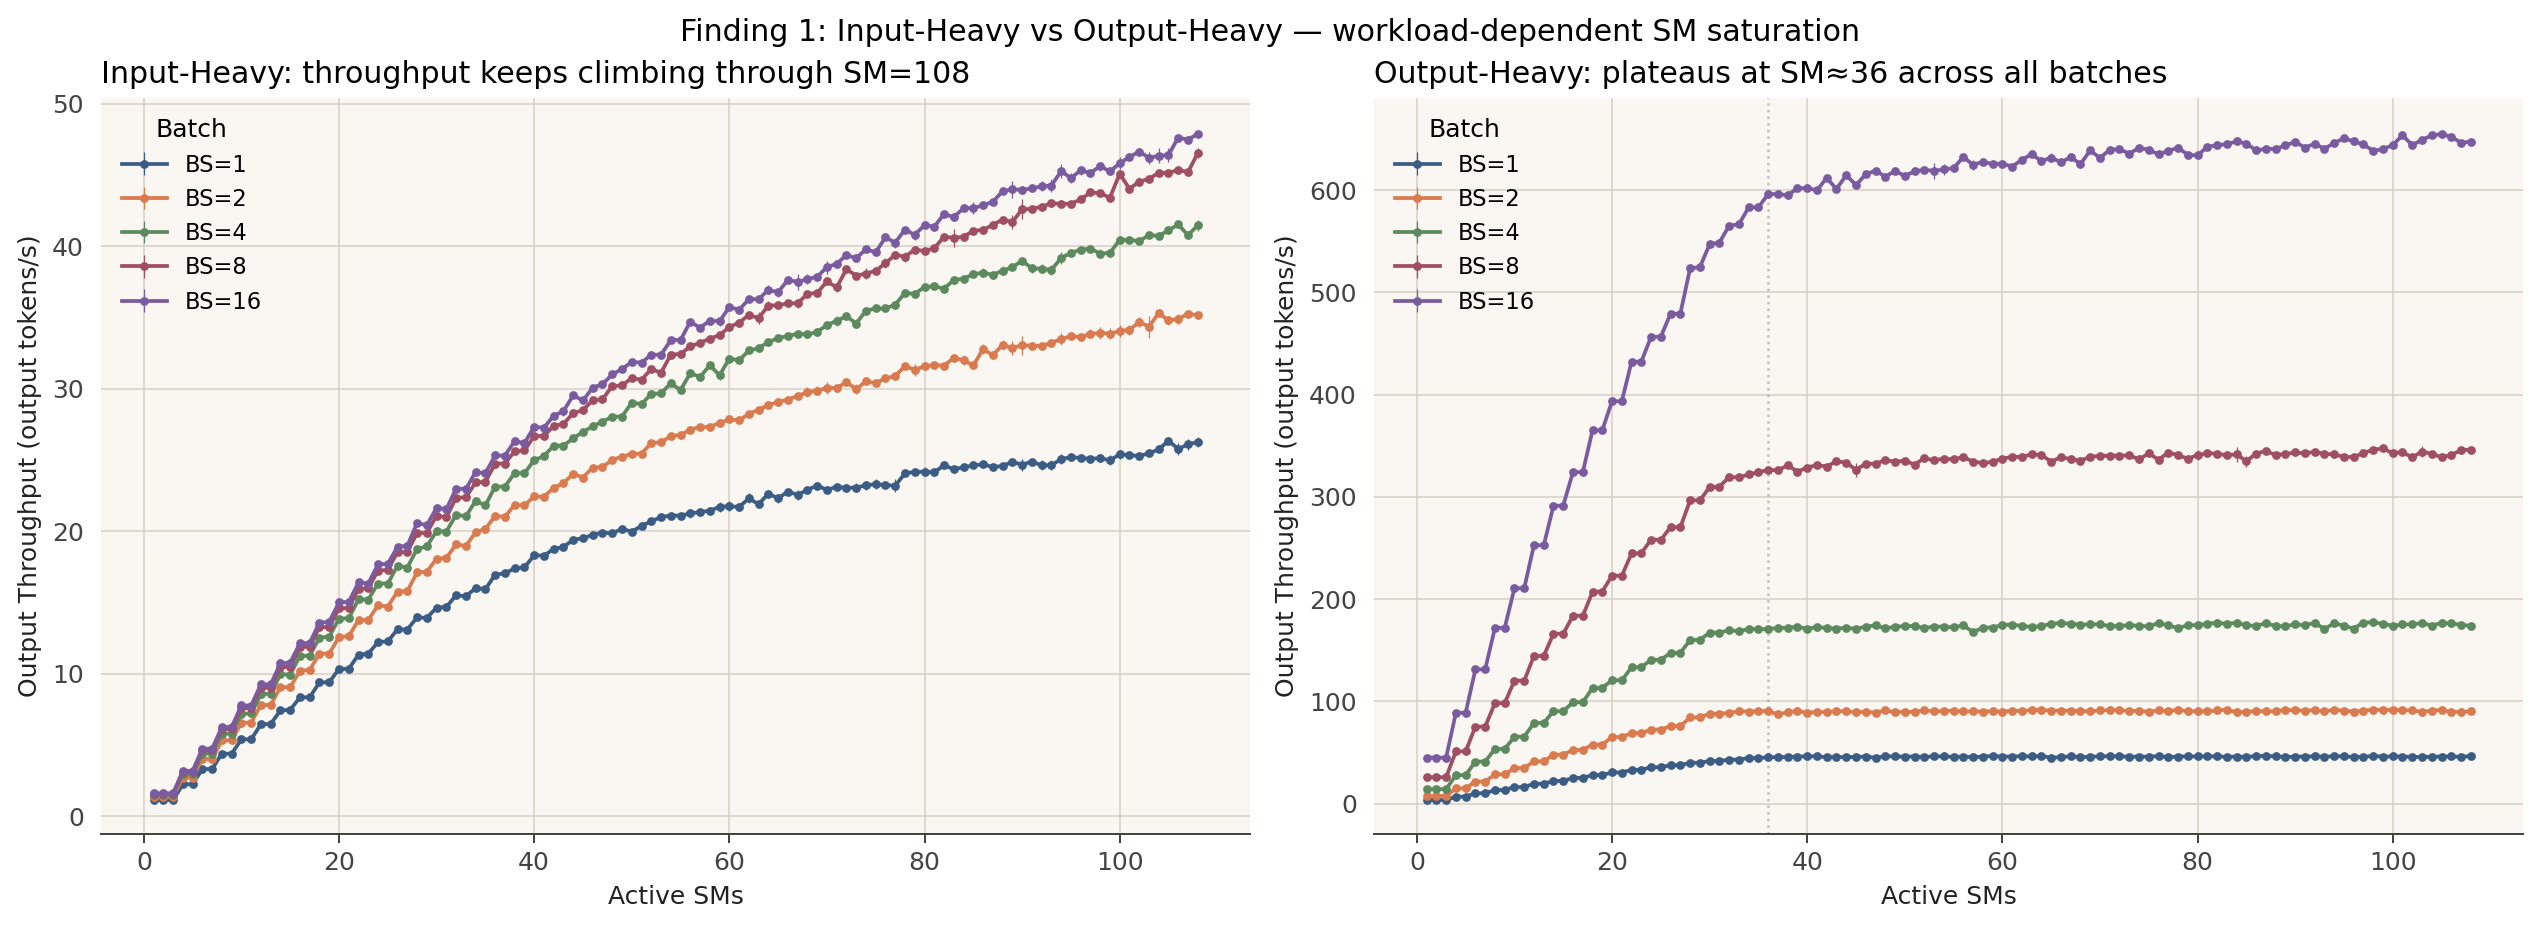
\includegraphics[width=\columnwidth]{figs/finding1_throughput_plateau.png}
    \caption{}
    \label{fig:throughput_scaling}
\end{figure}

\subsection{Throughput Saturates for Output Workload}
\label{sec:eval-throughput}

Figure~\ref{fig:throughput_scaling} shows output throughput as active SM count varies from 2 to 108 for both workload classes.

Output-Heavy throughput rises steeply at low SM count and then plateaus at approximately 36 active SMs across all batch sizes we tested. The plateau softens slightly at large batch sizes, but the elbow at SM$\approx$36 is consistent across all five batch configurations. This is evidence of a memory-bandwidth-bound workload.

Input-Heavy throughput scales differently. Across all batch sizes, throughput continues to climb through SM=108 with no plateau visible in the measured range. Input-Heavy spends more wall time in vision encoding and prefill, both of which are compute-bound and continue to extract value from additional SMs. Decode is a smaller fraction of the request, so its memory-bound saturation does not dominate the end-to-end curve.

\begin{figure}[t]
    \centering
    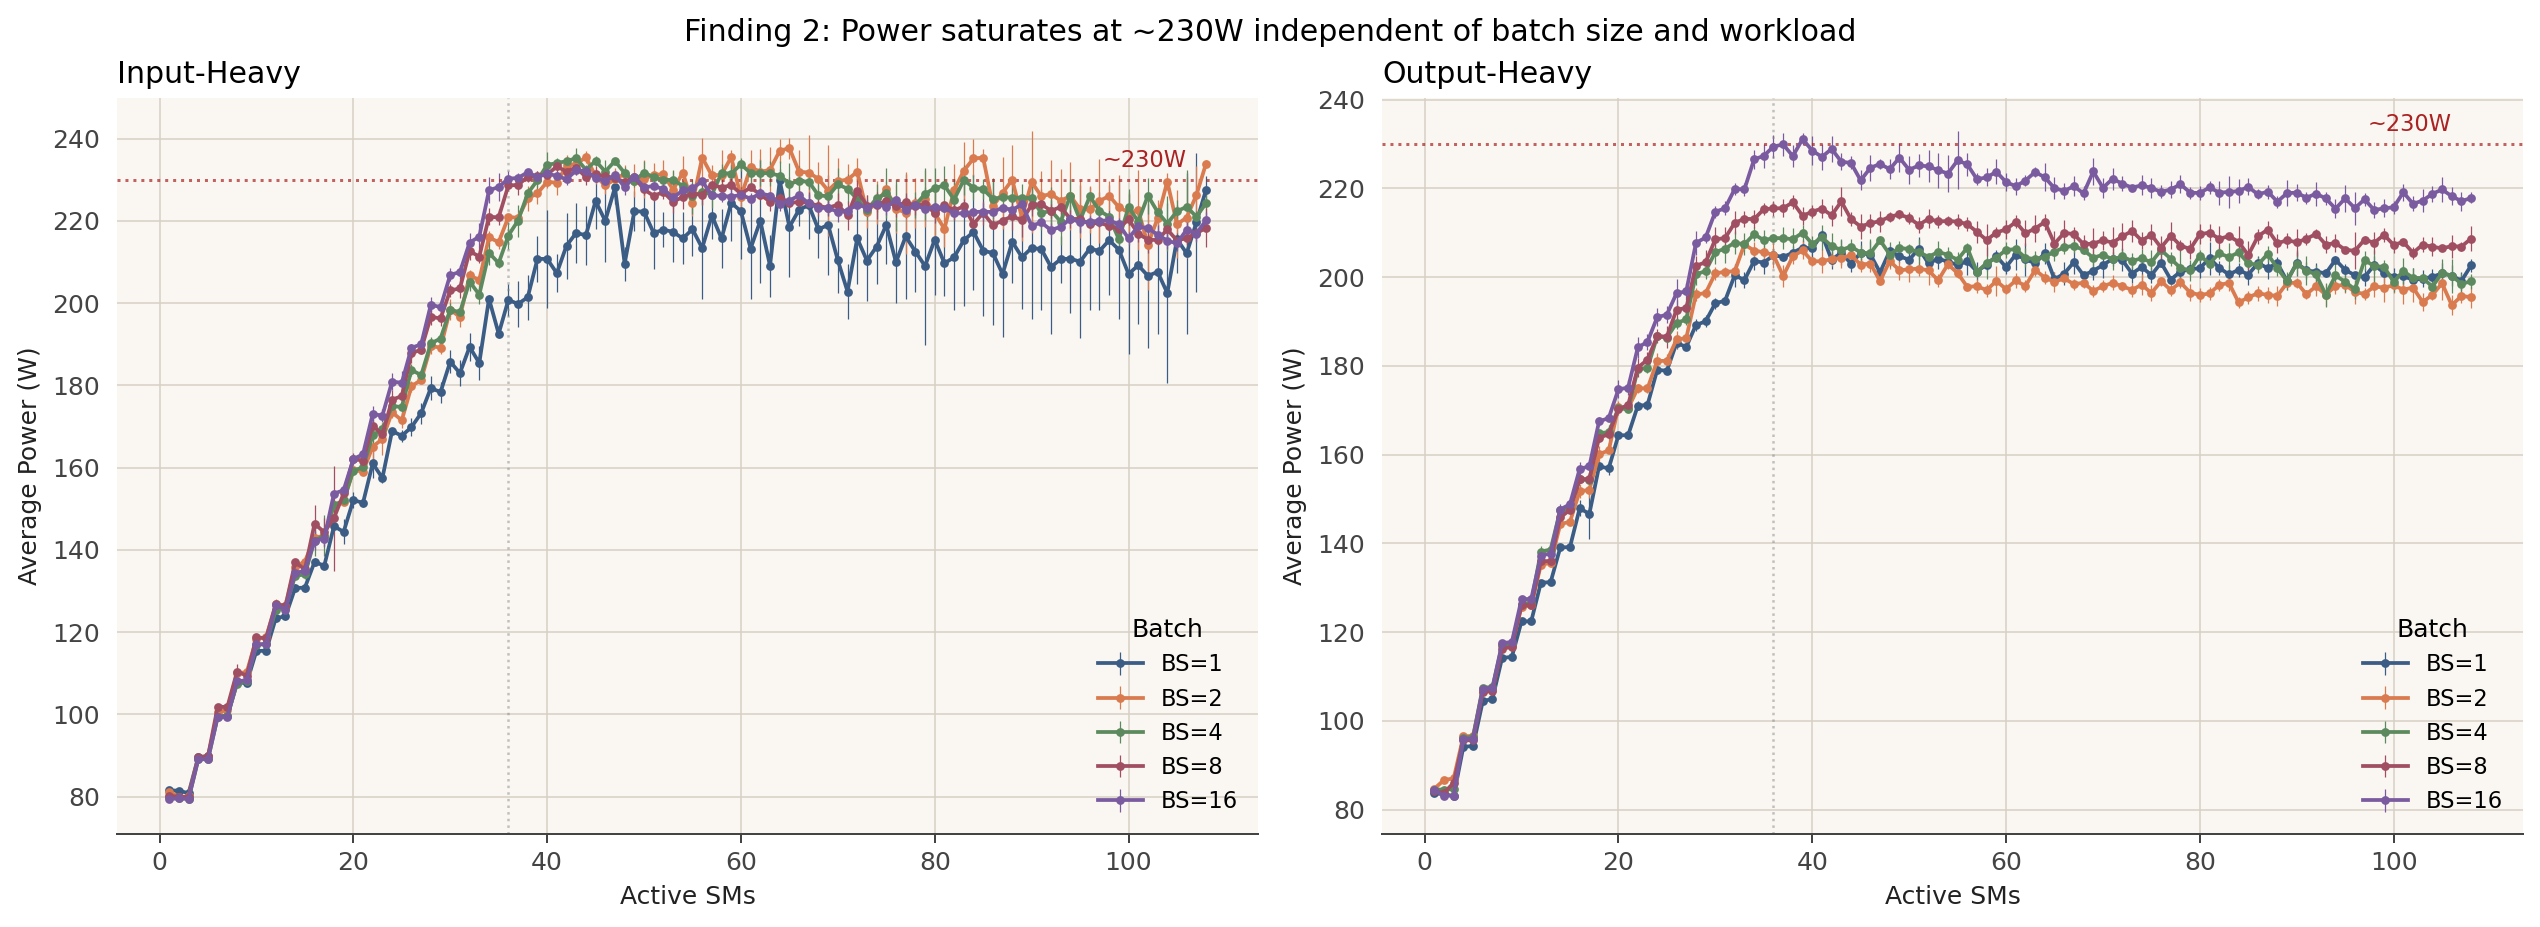
\includegraphics[width=\columnwidth]{figs/finding2_power_ceiling.png}
    \caption{}
    \label{fig:power_scaling}
\end{figure}

\subsection{Power Saturates Independent of Batch Size}
\label{sec:eval-power}

Figure~\ref{fig:power_scaling} shows average GPU power as active SM count varies. Across both workloads and all batch sizes, power rises linearly with SM count up to SM$\approx$36 and then flattens at a workload-dependent ceiling. For Input-Heavy and for Output-Heavy at batch sizes $\geq$4, power plateaus at approximately 230~W (A100 SXM4 TDP is 250~W). For Output-Heavy at batch size 1, the ceiling is lower at 203--210~W, reflecting the workload's inability to drive the GPU to full power even when given the entire chip.

The critical observation is that the SM count at which power saturates is the same threshold at which Output-Heavy throughput saturates. Above SM=36, Output-Heavy neither generates more tokens nor draws more power. The remaining 72 SMs are clocked, allocated to the workload, and contribute neither useful work nor measurable power consumption. 

\begin{figure}[h]
    \centering
    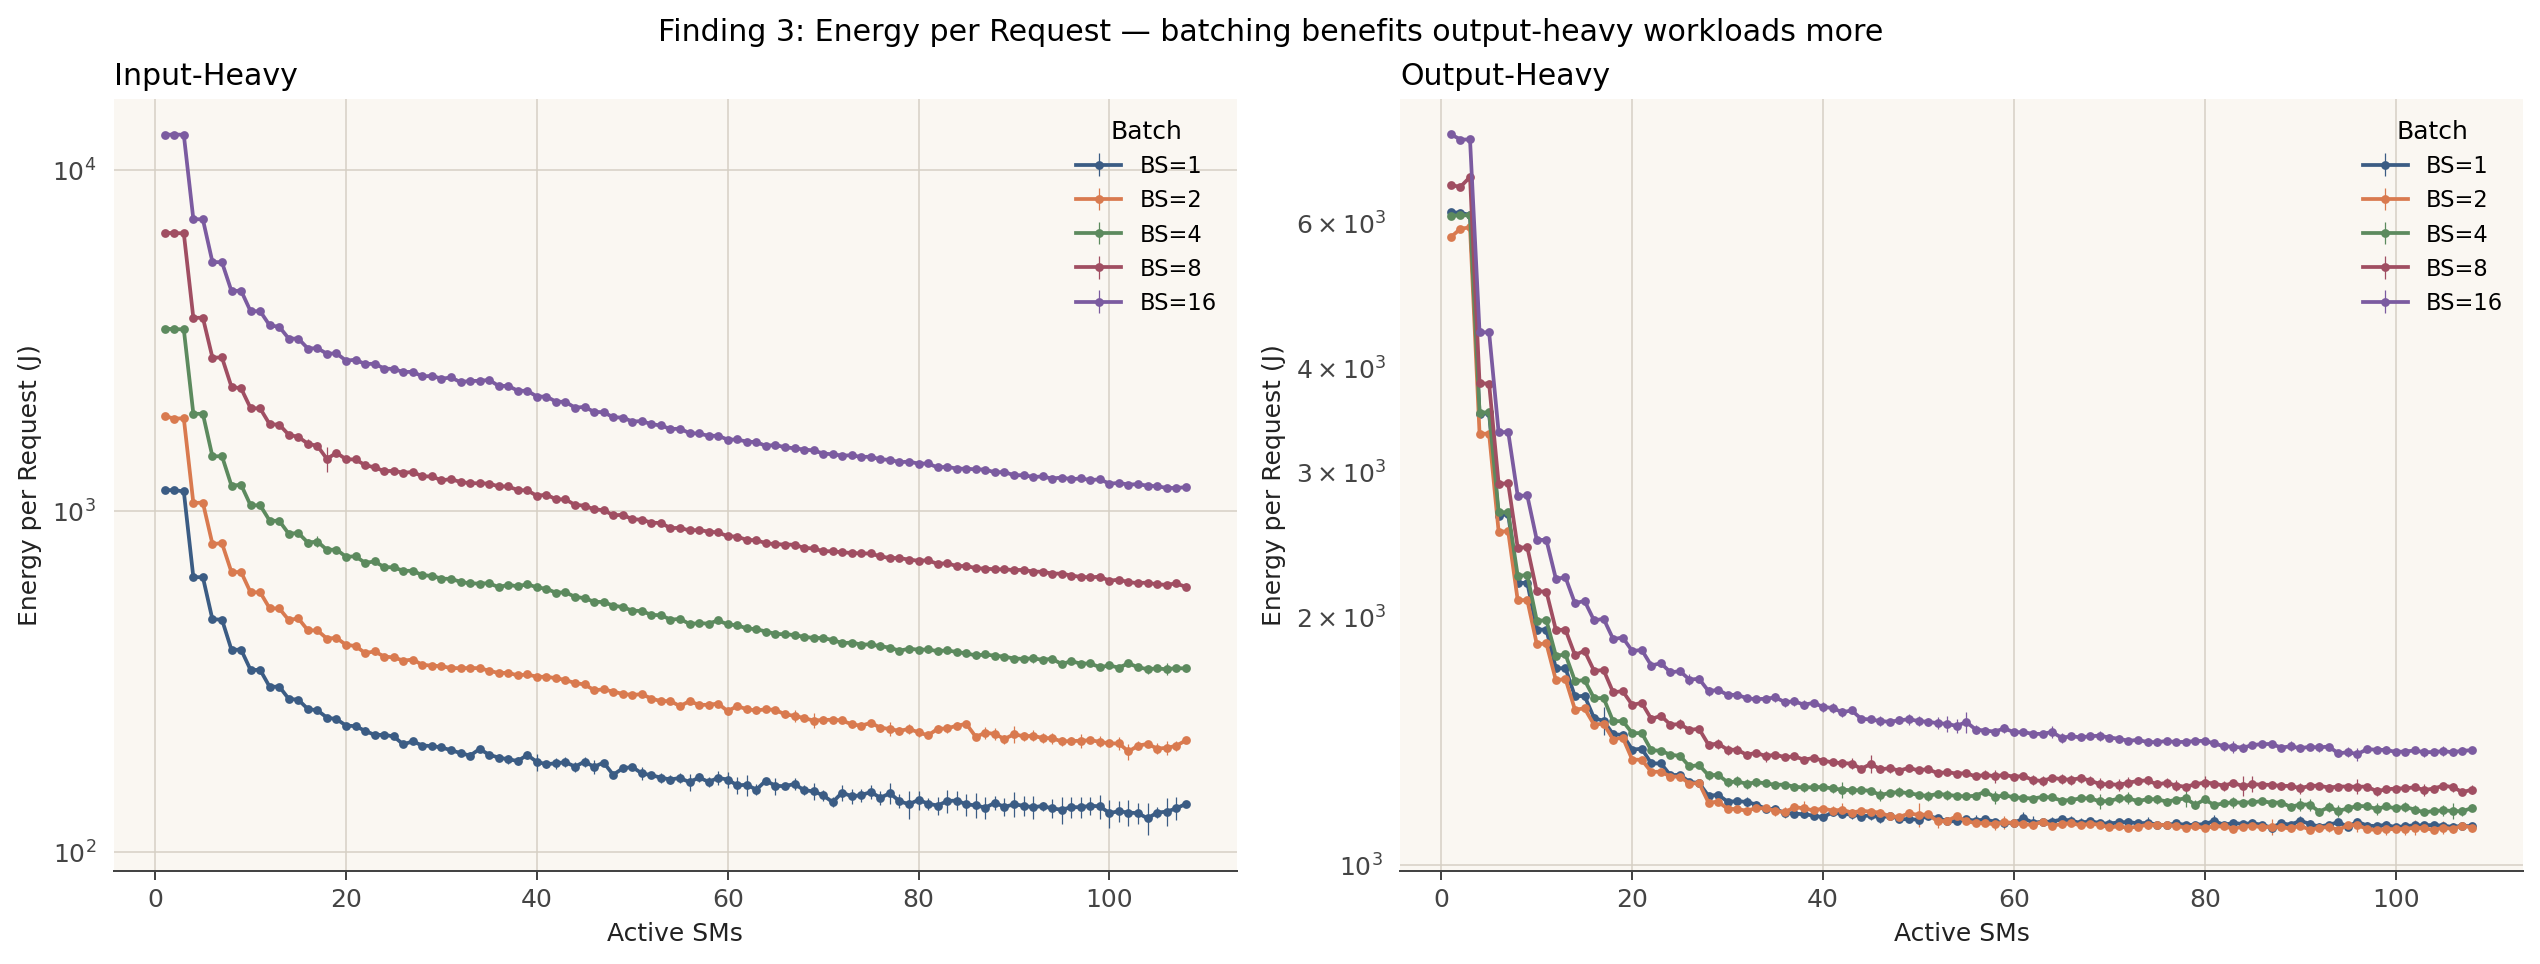
\includegraphics[width=\columnwidth]{figs/finding3_energy_per_request.png}
    \caption{}
    \label{fig:energy_scaling}
\end{figure}

\subsection{Batching Benefits Are Asymmetric Across Workloads}
\label{sec:eval-energy}

Figure~\ref{fig:energy_scaling} shows energy per request as a function of SM count for both workloads. We focus here on the comparison at SM=108, where each workload reaches its lowest per-request energy.

For Output-Heavy, energy per request increases by only 24\% from batch size 1 (1114~J/req) to batch size 16 (1378~J/req), even though the system serves 16$\times$ more requests in that batch (12.9$\times$ difference in energy per request). For Input-Heavy, the picture is very different: energy per request increases 8.5$\times$ from batch size 1 (139~J/req) to batch size 16 (1177~J/req) (1.9$\times$ difference in energy per request).

Input-Heavy requests pay a fixed vision encoder cost (approximately 1~s of encoder work for the $1344^2$ image) that does not amortize across the batch. Each additional request in the batch runs the encoder again, scaling the fixed cost roughly linearly with batch size. Output-Heavy requests, in contrast, run a much smaller encoder ($448^2$ image, 256 tokens) once per request and then spend most of their time in decode, where batching directly amortizes weight loads across concurrent sequences. Batching is a strong energy lever for output-dominated workloads and a weak one for input-dominated ones.

\subsection{Implications for SM Masking}
\label{sec:eval-implications}

The three findings above tell a consistent story about SM masking as an energy-saving technique for single-job MLLM serving.

Below the saturation threshold, masking SMs reduces throughput and power roughly proportionally, leaving energy per request approximately unchanged. Above the saturation threshold, masking the stranded SMs does not reduce power (given the limitation of TDP at 250W): the workload is already drawing as much power as it can drive on the SMs it actually uses, and the masked SMs were contributing little to that draw. In neither regime does single-job SM masking reduce energy per request below what the full GPU achieves. Across all 1{,}080 measured configurations, the lowest energy per request for each (workload, batch size) pair occurs at or near SM=108 where the full GPU is the most energy-efficient single-job configuration we measured.

This is a positive result for output-heavy workloads as its an obvious application to save energy by performing SM masking. The stranded capacity is there as 67\% of the GPU sits powered but unused during Output-Heavy decode at small batch sizes. Two unmasked knobs could plausibly recover it. First, frequency throttling during decode exploits the memory-bound regime. Second, cross-workload spatial multiplexing could place Input-Heavy compute work. We did not test either knob in this work; the data motivates them as the natural next directions.

\section{Future Work}

Several directions remain for extending this work into a fully phase-aware serving system.

First, we plan to evaluate concurrent execution across multiple models and workloads using spatial GPU partitioning. This would allow compute-heavy and memory-light phases to execute simultaneously while isolating their resource demands.

Second, we plan to study frequency scaling as a complementary optimization technique. Different inference phases may benefit from different GPU clock configurations depending on whether they are compute-bound or memory-sensitive.

Third, we plan to investigate memory partitioning techniques alongside SM partitioning to further isolate phase behavior and reduce interference between concurrent workloads.

More broadly, future serving systems must remain workload-sensitive. Input-Heavy workloads expose substantially different optimization opportunities than generation-heavy workloads. Effective systems will need to dynamically adapt resource allocation according to workload composition and inference phase behavior.

\section{Conclusion}

This work presents a phase-level characterization of multimodal LLM inference on modern GPUs. Across InternVL3-8B workloads, we find that Decode dominates runtime while substantially underutilizing both compute and memory bandwidth. In contrast, Vision Encoder, MLP Connector, and Prefill behave as significantly more compute-intensive stages.

Generation-heavy workloads in particular plateau at moderate SM allocations across throughput, latency, and power metrics, exposing substantial reclaimable compute headroom during Decode execution. Input-Heavy workloads instead continue scaling with additional compute resources and remain substantially more sensitive to constrained SM allocation.

These observations motivate phase-aware GPU resource allocation strategies that adapt hardware provisioning according to the needs of each inference phase rather than treating inference as a monolithic workload.

Overall, our results suggest that future MLLM serving systems can improve energy efficiency by dynamically partitioning GPU resources according to phase behavior while preserving competitive serving performance.

\balance
\bibliographystyle{IEEEtran}
\bibliography{refs}

\end{document}